\section{Achados da Pesquisa}

Para o estudo de caso, os dados obtidos nas entrevistas s�o apresentados de
acordo com a divis�o de grupo, cada grupo � apresentado e analisado
individualmente, permitindo assim, maior entendimento dos resultados obitidos.

Para melhor compreens�o, a an�lise � apresentada graficamente nas Figuras
\ref{img:graphdir}, \ref{img:graphger}, \ref{img:graphefe}, \ref{img:graphter},
\ref{img:graphcon}.

%%% Inserir Graficos aqui
\newlength{\imgwidth}
\setlength{\imgwidth}{16.09cm}
\newlength{\imgheight}
\setlength{\imgheight}{10.59cm}

\begin{figure}[H]
  \centering
	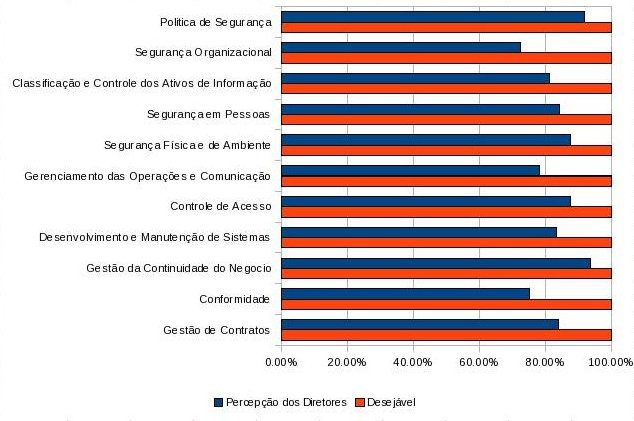
\includegraphics[height=\imgheight,width=\imgwidth]{graph_dir}
  \caption{Resultado {--} Percep��o dos Diretores}
  \label{img:graphdir}
\end{figure}

\begin{figure}[H]
  \centering
	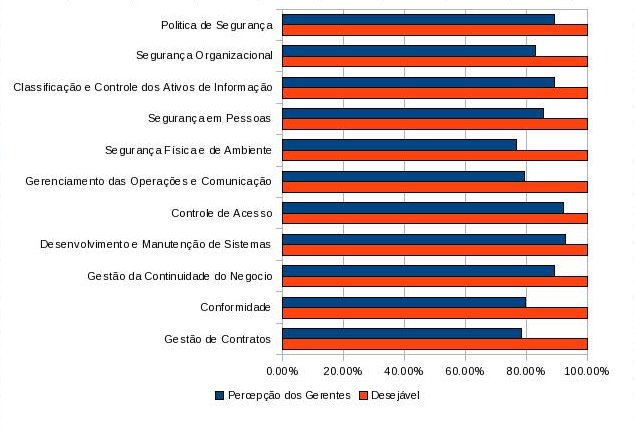
\includegraphics[height=\imgheight,width=\imgwidth]{graph_ger}
  \caption{Resultado {--} Percep��o dos Gerentes}
  \label{img:graphger}
\end{figure}

\begin{figure}[H]
  \centering
	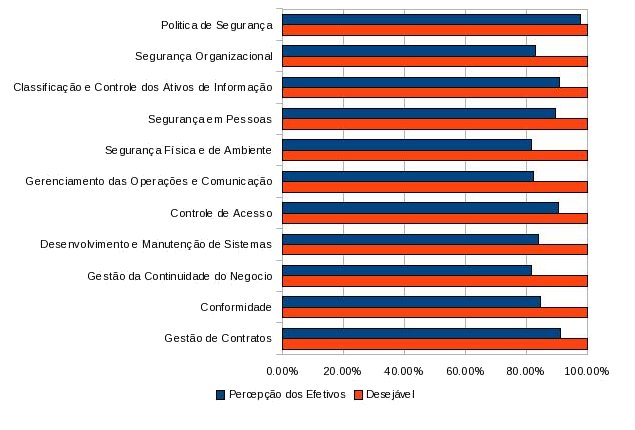
\includegraphics[height=\imgheight,width=\imgwidth]{graph_efe}
  \caption{Resultado {--} Percep��o dos Funcion�rios Efetivos}
  \label{img:graphefe}
\end{figure}

\begin{figure}[H]
  \centering
	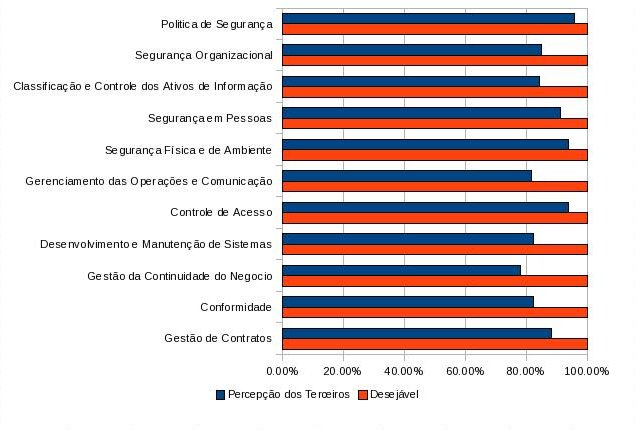
\includegraphics[height=\imgheight,width=\imgwidth]{graph_ter}
  \caption{Resultado {--} Percep��o dos Terceiros}
  \label{img:graphter}
\end{figure}

\begin{figure}[H]
  \centering
	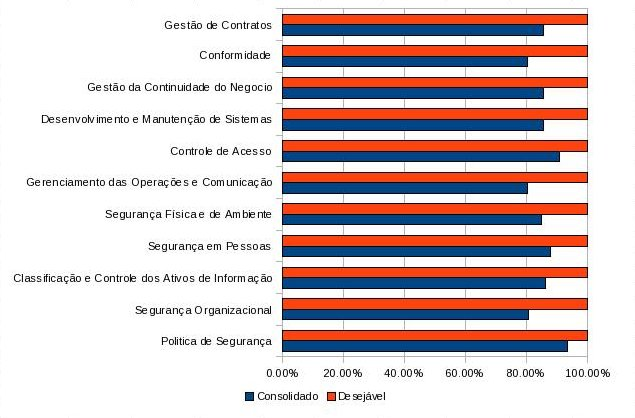
\includegraphics[height=\imgheight,width=\imgwidth]{graph_con}
  \caption{Resultado {--} Percep��es Consolidadas}
  \label{img:graphcon}
\end{figure}

\clearpage

